\documentclass{article} %default font size is 10, to specifiy other sizes use \documentclass[12pt]{article} %to have the  numbers on the left for equations use \documentclass[12pt,leqno]{article} % to have landscape pages to accomdate large tableaus \documentclass[landscape]{article}

%Documents used to put this together: examples.tex,  lshort030331.pdf

%------Perhaps outdated--------------------------------------------

%Create asii text blocks, often used to indicate something is code:
%Check to see if this is necessary
\usepackage{verbatim} 

%Show how an unknown word can be hyphenated throughout the document.
	\hyphenation{so-lil-o-quy}

%\syntonly %if this is uncommented this command to make the tex go faster it just checks syntax not make a new dvi file.

%-----General Needs------------------------------------------------

%Standard printing is little centered booksized pages, this makes it a full letter page
	\usepackage{fullpage}
	
%Print 2 pages on 1 page (this is one way to do it)		
	%\usepackage{2up}

%Underline and Strikeout capabilities (sideeffect: \emph changes from the default italics to underline, to avoid this use \textit for italics)
% this also makes ugly underlines in the bibtex references
	%\usepackage{ulem} use \sout

	
%Display images	
	\usepackage[dvips]{graphicx} % you must save the file as a eps, or ps.  to display the image type this: \includegraphics{filename} 


%Bibliography:
	\usepackage{natbib} %citation style
	\bibpunct{(}{)}{;}{a}{,}{,}
	%\bibliographystyle{plainnat}
	\bibliographystyle{linquiry2}
	

%A way to make an index
\usepackage{makeidx}
\makeindex



%-----Begin Linguistics Packages----------------------------------

%Syntax/Morphology Intralinear glosses:
	\usepackage{covington}
	
	%complicated package (relatively new!) with lots of features and a whole new way of thinking about trees
	\usepackage{pst-jtree}
	\usepackage{xkeyval}

%Easy tree structures based off of brackting:
	%\usepackage{qtree} 
	\usepackage{qtreegina} %changes: the original qtree is incompatible with xyling because both use the command \Tree, so i changed qtree so that it uses \QTree instead, now qtreegina and xyling are compatible
	
%Arrows for the qtree easy tree structures
	%\usepackage{tree-dvips}

%Complicated tree structures and much more
	%\usepackage{xyling}
	\usepackage{xylinggina} %changes: i added text arrows that go over the text. not an important change, so most people can use xyling instead.

%IPA fonts
	\usepackage{tipa}
	\let\ipa\textipa %this command allows you to use the shorter \ipa{} rather than the longer \textipa{}

%Semantics denotation double brackets
	%this declares some new commands \denote{} and \denoteexpand{} to get semantics denotations that are easier to use than the stmarysrd package.
	\newcommand{\denote}[1]{[\hspace{-.02in}[{\bf #1}]\hspace{-.02in}]}
	\newcommand{\denoteexpand}[1]{$\left[\hspace{-.06in}\left[#1\hspace{-1in}\right]\hspace{-.06in}\right]$}
	
	
	%Create diagrams (set theory,)
	\usepackage{pstricks}
	\usepackage{pst-grad}
		%inorder to set the unit size add this before the item \psset{unit=3em}
	
	
%Phonology
	%to create a vowel space
	\usepackage{vowel}


%Otimality Theory
	%to get a hand for the tableau
	\usepackage{pifont}
	%declares the command \hand that accesses the dingbat 43
	\newcommand{\hand}{\ding{43}}
	%to shade in tables
	\usepackage{color}
	\usepackage{colortab}
	\definecolor{lightgray}{gray}{0.8}
	
	
	%to make long tables spaning a number of pages
	\usepackage{supertabular}
	%to make landscaped pages add [landscape] in the \documentclass[landscape]{article}
	
	
	%\usepackage[frenchb]{babel}
	%the french bable makes it possible to use the ranking symbols which are actually french quotes \fg \og, but this effectively makes it a french document, which has effects on the spacing of  the colon : and other changes in the document structure. so instead i defined some commands, which are accessed by \fg and \og:
	\newcommand{\fg}{{\raisebox{0.28ex}{\tiny $>$}}\hspace{-.06in}{\raisebox{0.1ex}{\scriptsize $>$}}}
	\newcommand{\og}{$<\hspace{-.06in}<$}

%Autosegmental phonology represenations
	\usepackage{pst-autoseg} %this appears to reset the spacing in the pstricks and set theory graphics... to fix that type \psset{unit=3em} to set the unit spacing

%Precedence theory?
	%\usepackage[curve]{xypic}incompatible with xyling i think? xyling is based off of xy or xypic
%-------Miscellaneous---------------------------------------------

	%\usepackage{marvosym} for smilie
	%\usepackage{latexsym}
	%\usepackage{eepic}
	%\usepackage{pst-eucl}
	%\usepackage{SpecialCoor}

%--------------------End Preamble Area-----------------------------

\begin{document}
%\pagenumbering{roman} %makes the numbering of the preface material in roman numerals
	%Calling the pavgenumbering command in teh middle of hte documetn has the pages start over again. the style can also be changed for example the table of contents can be in roman and the rest of the document can be in arabic. and the appendix can be in capital Roman letters etc...
%\pagestyle{myheadings}
	%\markboth{left-hand (even)page header}{Right-hand (odd) page header}
	%in the book format because its default is doublesided printing you can have different headigns for the right and left hand pages. use \markboth to do this. otherwise you can just use \markright
\title{Latex for Linguistics Notes\thanks{Acknowledgments: tons and tons of other latex for linguists websites and tutorials}}
\author{Gina \and Author2}
\date{v1 May 25th 2003\\ v2 Feb 24 2008}%if the \date command is omitted the current date is used or the command \today can be used (anywhere in the document)
\maketitle

%the table of contents is very useful in planning a document. it can serve as an outline both for the author, and for the reviewers until the final version where it maybe preffered to not display it. 
\tableofcontents
%\clearpage %this makes the text go on the next page, handy with real tables of contents


%-------------------End Heading Area-------------------------------

\abstract{This is an abstract of what this paper is about. This collection of latex source started in 2003 from reading a LaTEX for Everyone by Jane Hahn (published in 1993).  Since then, a number of commands had changed in \LaTeXe{}. This document contains the latest commands  (to my knowledge) as of Feb 2008. This document is designed to contain tons of Latex examples that a linguist can copy and paste into their own documents, it should also help with a bit of theory so you can learn how to get the packages you need to run the code, and you can learn how to  tweek the example code by looking up the documentation for those packages, or for LaTeX in general. It should get you up and running as a good mentor should. As you read the .pdf output of this .tex file you can bounce back and forth between the output (.pdf) and the source (.tex) to see how the output was coded. LaTeX is certainly one of the easiest programming languages you can learn. Essentially,  almost all latex comands are 1 place predicates that start with a slash and take one obligatory argument in curly braces \{arg\} and perhaps optional (comma seperated) arguments in square brackets [arg1,arg2,arg3], take a look at the code to see some examples}

\begin{quotation}Alternatively, you can make an abstract like this (see source). blah blah blah blah blah blah blah blah blah blah blah blah blah blah blah blah blah blah blah blah blah blah blah blah blah blah blah blah blah blah blah blah blah blah blah blah blah blah blah blah blah blah blah blah blah blah blah blah blah blah blah blah blah blah blah blah blah blah blah blah blah blah blah blah blah blah blah blah blah blah blah blah blah blah blah blah blah blah blah blah blah blah blah blah blah blah blah blah blah blah blah blah blah blah blah blah blah blah blah blah blah blah blah blah
\end{quotation}

%\setcounter{page}{1}
%\pagenumbering{arabic} %brings numbering back to the default

\part{Instalation}
\section{How to use LaTeX}

You can use Latex on Windows, MacOS and Linux.

LaTeX is a type of programming language for formating scientific texts/books. It's not a Word Processor (like Microsoft Word, WordPad or WordPerfect). In fact, all word processers save their documents in a code that is readable by that application. LaTex is like this code, its a level deeper than what you view, and allows you more control over the document than a Word Processor. 

LaTex makes it very easy to draw uniform diagrams and write forumlas using plain text. If you already know a bit about HTML or any other programming language this will be easy for you.

There are 3 steps to making a file in LaTeX.

\begin{itemize}
   \item Edit a plain text file.
   \item run LaTex to proccess the file.
   \item view the output (there are three formats for the output, dvi, ps, pdf. there are differences that will be discussed later). 
\end{itemize}

After you are finished your document it will exist as a .pdf 

LaTex began on the Linux operating system. So the installation for Linux users is very common and there are plenty of explainations online. Similarly Mac OS X is actually based off of Linux, so its also common to install Latex on a Mac. 


\subsubsection{Linux Instalation}

teTex is no longer supported (2006) instead use texlive.

create a user directory to put your own sty files


cd ~
mkdir -p texmf/tex/latex/foo

Now, we must make LaTeX recognize the new package:

texhash ~/texmf

\subsection{Windows instalation}
Since running Latex on Microsoft Windows is the most complicated, I will explain a way to install LaTeX on a MS Windows machine. (If you have a Mac you can try http://www.esm.psu.edu/mac-tex/)



Getting \LaTeX to run on windows can be annoying. As of March 2008 here is something that works:

\begin{itemize}
	\item Download MikTex (the distribution of LaTeX for windows, for linux its teTeX, for Mac its XeTeX or something like that), 
		\begin{itemize}
			\item download and open a file similar to setup-2.7.2904.exe This file is both for downloading, and for installing. 
			\item First choose the Download MiKTex, then choose Basic (it takes less time to download) or choose Complete (this is better if you can do it, because you will have less problems installing packages later) 
			\item Choose a source to download from (the sources in the united states are not reliable and quit downloading in the middle, the sources from canada and austria work pretty well. if the source stops downloading in the middle you can just repeat the same process and it will skip the files that it has already sucessfully downloaded and continue to download where it left off.)
		\end{itemize}
	\item Install MikTex using the same file as before: setup-2.7.2904.exe
	\item Install an IDE (Integrated Development Environment) a centralized place to edit your LaTex source, and view the output(s) in DVI, PS or PDF format. There are two options I know about: TeXnicCenter (a file named something like TXCSetup\_1Beta7\_01.exe) and TexMaker, but I've had far more errors and trouble using TexMaker, so I like TeXnicCenter better. 
	\item Install Ghostscript and Ghostview (do an internet search for them and how to install them)
	\item Open a .tex file using the IDE (TeXnixCenter), browse around and try to latex it 
	\item Install packages that you need (often if you need a package a box will pop up when you latex the file which will ask you to download the file. This might work. But, a surefire way to install packages is to go to $Start>>Programs>>MiKTeX>>Browse Packages$ )
	\item If you have packages that you want to use, but they aren't downloadable (ie, you made them or someone else made them) then you can go  $Start>>Programs>>MiKTeX>>Settings$ again you should browse around and become familiar with the options. Choose the Roots tab, this is a list of directories where the packages (.sty files) can be saved. Basically you can put your .sty files into C:\\Local TeX Files , then go the General tab in the Settings box, and click on Refresh FNDB (this refreshes the database of packages, and it should find your new packages)
	\item Try editing your .tex document, and viewing it. You might have to explore around the IDE (TeXnicCenter) to find out how to do a spell check, how to latex the document, how to view the document, and how to change your output between  DVI, PS and PDF.
\end{itemize} 

(Note, this advice is old, from 2003 and might not be true anymore.) There are basically 4 stages to get from a .tex file to the .pdf that you can distribute. 
\begin{itemize}
	\item Latex the file into a DVI (Device Independent Format) \\now the output is viewable with Yap
	\item dvips the file from dvi to ps (Post Script, a langauge that printers can read, the predecesor of pdf) \\now the output is viewable with Ghost View
	\item distill/print the document from ps to pdf (Portable Document Format) \\now the output is viewable with Adobe Reader/Professional
\end{itemize}

These extra stages have been recently bypassed using pdfTex. This makes a better pdf using modern pdf features. But, linguists use a number of packages that use ps specials (specials are arrows and lines) that can only be displayed in ps, which are then converted into images when the document is made as a pdf. 

So, for most linguistics papers we are forced to go through the 4 stages of output. If you ever have arrows and graphics that dont show up, (or error messages like ``Non-PDF special ignored!'') chances are youre using pdfTex, and you need to change some options in your IDE to get it to go through all the dvi and ps stages. You can still view the document, you will just be missing the fancy specials...

\part{Using LaTex}



\section{Here is a Section}
	\label{sec:sectioningExample} 

In this section (Section~\ref{sec:sectioningExample}) we will first see how to make sections (in \ref{sec:sectioningExample}), subsections (in \ref{sec:subsectionExample}) and subsubsections (in \ref{sec:subsubsectionExample}). In \S \ref{sec:messingWithSectioning} we will see some more advanced tools for sectioning. 

\subsection{This is a subsection}
	\label{sec:subsectionExample}


    `Twas brillig, and the slithy toves
    Did gyre and gimble in the wabe:
    All mimsy were the borogoves,
    And the mome raths outgrabe.


    ``Beware the Jabberwock, my son!
    The jaws that bite, the claws that catch!
    Beware the Jubjub bird, and shun
    The frumious Bandersnatch!"
    
\subsubsection{This is a subsubsection}
	\label{sec:subsubsectionExample}

    He took his vorpal sword in hand:
    Long time the manxome foe he sought--
    So rested he by the Tumtum tree,
    And stood awhile in thought.
    
%\subsubsubsection{There is no such thing as a subsubsubsection}	    
    
    And, as in uffish thought he stood,
    The Jabberwock, with eyes of flame,
    Came whiffling through the tulgey wood,
    And burbled as it came!

    One, two! One, two! And through and through
    The vorpal blade went snicker-snack!
    He left it dead, and with its head
    He went galumphing back.

\subsubsection{Paragraphs and subparagraphs}

This is just about the headings use of pharagrahs. The spacing of pharagraphs is discussed in \S \ref{sec:spacing}.

\paragraph{This is a paragraph}

    ``And hast thou slain the Jabberwock?
    Come to my arms, my beamish boy!
    O frabjous day! Callooh! Callay!"
    He chortled in his joy.
    
\subparagraph{This is a subparagraph}

    `Twas brillig, and the slithy toves
    Did gyre and gimble in the wabe:
    All mimsy were the borogoves,
    And the mome raths outgrabe. 



\subsection{Advanced Sectioning: Section headings are automatically displayed in the table of contents}
	\label{sec:messingWithSectioning}

You must always tex a document twice in order to get a correct table of contents, and to get the references to be correctly evaluated. 

The table of contents will be displayed where you use the command {\verb \tableofcontents }. 


~\\
Although sections are automatically put in the Table of Contents (TOC), there are three things you can do to change this.

\begin{itemize}
	\item You can use section headings as just headings (that dont appear in the TOC and dont have a number)  with {\verb \section*{JustAHeading} }
	\item You can specify an optional arugment for the section's TOC entry (to modify/shorten a section heading) with {\verb \section[ShortVersion]{FullVersion} }
	\item You can add a non-numbered line\footnote{The addcontentsline must appear on the same page as the unnumberd heading inorder to have the right page number in the table of contents.}  in the TOC (to indicate a new Part) \\
	with {\verb \addcontentsline{toc}{section}{PartII:} }
\end{itemize} 


\addcontentsline{toc}{subsection}{Part II: But you can mess with the Table Of Contents and Headings}

\subsubsection*{But this subsection will have no number and serves as a heading}

	To make a simple heading you can add an asterix in the code between the command and its argument (see code).

\subsubsection[Short for TOC: Occams Razor and more]{Long: Occams greatest Razor and Shaving Cream}

	This section's TOC entry is different from its heading in the text. The TOC entry is specified in an [optional argument] (see code).

\section{Cross Referenecs}

	References {\verb \ref{} }  (not to be confused with a bibliography) will take the number of the example or section that their corresponding {\verb \label{} } command is located after (look for some examples in the code). You can also do {\verb \pageref{} } For example, spacing is discussed on page~\pageref{sec:spacing}.

	Counters can be reset (counters: part, chapter, section, subsection, subsubsection, paragraph, page, equation, figure, table, footnote, enumi, enumii). See the source between the table of contents and document body, and between the body and the appendix. 
	
	You can create your  own counter with newcounter, do an internet search for more info.  % more info: http://www.personal.ceu.hu/tex/counters.htm 
	
	It helps to name your labels with a prefix depending on what they are, ie a section as sec: or example as ex: (see code for examples).

\section{How Spacing Works in LaTeX}\label{sec:spacing}


\subsection{Basic Spacing: spaces, paragraphs, tabs}	

	\LaTeX ignores spacing in your source code, it handles all the spacing for you.  	Ignoring the spacing in code is actually useful, it means you can space your code so that it is easy to read. 

	\begin{example}\label{ex:forcespacing}
	Summary of Spacing, and ways to force it\\
	\begin{itemize} 
		\item Any number of blank lines will make a new paragraph (use  {\verb \\ } force a paragraph)
		\item Indentation is handled automatically (use {\verb \noindent } to force no indentation)
		\item Any number of spaces will make 1 space (use {\verb ~ } to force a space)
		\item Tabs are completely ignored. (use {\verb ~~~~~~or\hspace{.3in} } to force a tab)
	\end{itemize}
	\end{example}
	
	The tilda is also useful for things like \S~1, Section~1, Generalization~1, Figure~1, Example~1 where you dont want the `Example' and the `1' to be seperated by a line break (see code).

	
	\noindent You can get a single line break\\like this\\and this. 


\subsection{Indentation: Using quote and quotation}	
	
	The formated output (\ref{ex:formated}) was created with forced spacing. The unformated output (\ref{ex:unformated}) is what it looks like with no forced spacing: 
	

	\begin{example}\label{ex:unformated}
	Here is what an unformated `Le Jabberwock' looks like:\\ 
	
	Il \'{e}tait grilheure; les slictueux toves
	Gyraient sur l'alloinde et vriblaient:
	Tout flivoreux allaient les borogoves;
	Les verchons fourgus bourniflaient.
	
	``�Prends garde au Jabberwock, mon fils!
	A sa gueule qui mord, \`{a} ses griffes qui happent!
	Gare l`oiseau Jubjube, et laisse
	En paix le frumieux Bandersnatch!�"
	
	Le jeune homme, ayant pris sa vorpaline \'{e}p\'{e}e,
	Cherchait longtemps l`ennemi manziquais...
	Puis, arriv\'{e} pr�s de l`Arbre T\'{e}p\'{e},
	Pour r\'{e}fl\'{e}chir un instant s'arr\^{e}tait.
	
	Or, comme il ruminait de suff\^{e}ches pens�es,
	Le Jabberwock, l`oeil flamboyant,
	Ruginiflant par le bois touffet\'{e},
	Arrivait en barigoulant.
	
	Une, deux! Une, deux! D'outre en outre!
	Le glaive vorpalin virevolte, flac-vlan!
	Il terrasse le monstre, et, brandissant sa t\^{e}te,
	Il s`en retourne galomphant.
	
	``�Tu as donc tu\'{e} le Jabberwock!
	Dans mes bras, mon fils rayonnois!
	O jour frabieux! Callouh! Callock!�"
	Le vieux glouffait de joie.
	
	Il \'{e}tait grilheure; les slictueux toves
	Gyraient sur l`alloinde et vriblaient:
	Tout flivoreux allaient les borogoves;
	Les verchons fourgus bourniflaient.	
	\end{example}

	
	\begin{example} \label{ex:formated}
	Here is what `Le Jabberwock' should look like. \\
	
	\begin{quote}
		`Le Jabberwock' \\
		Translated by Henri Parisot: \\
		http://www.keithlim.com/jabberwocky/translations/index.html\\
		~\\
		Il \'{e}tait grilheure; les slictueux toves\\
		Gyraient sur l'alloinde et vriblaient:\\
		Tout flivoreux allaient les borogoves;\\
		Les verchons fourgus bourniflaient.\\
		~\\
		``�Prends garde au Jabberwock, mon fils!\\
		A sa gueule qui mord, \`{a} ses griffes qui happent!\\
		Gare l`oiseau Jubjube, et laisse\\
		En paix le frumieux Bandersnatch!�"\\
		~\\
		Le jeune homme, ayant pris sa vorpaline \'{e}p\'{e}e,\\
		Cherchait longtemps l`ennemi manziquais...\\
		Puis, arriv\'{e} pr�s de l`Arbre T\'{e}p\'{e},\\
		Pour r\'{e}fl\'{e}chir un instant s'arr\^{e}tait.\\
		~\\
		Or, comme il ruminait de suff\^{e}ches pens�es, \\
		Le Jabberwock, l`oeil flamboyant,\\
		Ruginiflant par le bois touffet\'{e},\\
		Arrivait en barigoulant.\\
		~\\
		Une, deux! Une, deux! D'outre en outre!\\
		Le glaive vorpalin virevolte, flac-vlan!\\
		Il terrasse le monstre, et, brandissant sa t\^{e}te,\\
		Il s`en retourne galomphant.\\~
		~\\
		``�Tu as donc tu\'{e} le Jabberwock!\\
		Dans mes bras, mon fils rayonnois!\\
		O jour frabieux! Callouh! Callock!�"\\
		Le vieux glouffait de joie.\\
		~\\
		Il \'{e}tait grilheure; les slictueux toves\\
		Gyraient sur l`alloinde et vriblaient:\\
		Tout flivoreux allaient les borogoves;\\
		Les verchons fourgus bourniflaient.\\
	\end{quote}
	\end{example}
	

	The formated output (\ref{ex:formated}) was created using quote. If you want to make a paragraph quotation you can use quotation
	
	\begin{quotation}
	
		%This immediately raises the question of how one can judge the theoretical significance of a given fact or body of facts. The answer is that this can be done by showing that the facts in question can be accounted for as consequences of laws organized in a well articulated theory\ldots
		\noindent  Unfortunately, within linguistics it has not been generally recognized how important such formal, theoretical work is; instead  there is a feeling that too much concern for theoretical detail is  a waste of time\ldots [T]he attitude that formal, theoretical work  is bound to be both ad-hoc and sterile is, I am convinced,  fundamentally mistaken \ldots 
		
		\index{hspace} \hspace{3in}Morris Halle (1975:530)
	\end{quotation}


	
\subsection{Advanced Spacing: vspace \index{vspace} and \index{hspace} hspace}\label{sec:advspacing}

You can create vertical space 

	\vspace{.6in} \index{vspace} like this. You can create horizontal space \hspace{.6in} like this. This can be useful in graphics, figures and examples. hspace can be useful in getting Trees to be smaller... but vspace and hspace are hacks that are best avoided and can have bad consequences.
	


\section{Lists and Enumeration}

\subsection{Enumerated Lists}

There are only four levels of list available. You can have an itemize list inside of an enumerated list and vice versa. See Item~\ref{list:level2}, Item~\ref{list:level3}, Item~\ref{list:level4} for examples of using references in lists.

Here is the automated way enumerated lists look

\begin{enumerate}
	\item This is the first level
	\begin{enumerate}
		\item \label{list:level2} This is the second level
		\begin{enumerate}
			\item \label{list:level3} This is the third level
			\begin{enumerate}
				\item \label{list:level4} This is the fourth level
			\end{enumerate}
		\end{enumerate}
		\item This is the seecond item in the second level
	\end{enumerate}
	\item This is the second item in the first level
\end{enumerate}

\subsection{Itemized Lists}

Here is the way that a normal itemized list looks. You change the bullet symbols to anything you want.

\begin{itemize}
	\item here is a bunch of embedded items
	\item buy groceries
	\begin{itemize}
		\item potatoes
		\begin{itemize}
			\item red
			\begin{itemize}
				\item russet
			\end{itemize}
			\item yellow
		\end{itemize}
		\item celery
		\item frying chicken
		\item milk
	\end{itemize}
	\item[o] Here is a changed example pay bills
	\item [$\heartsuit$] Here is a changed example do laundry
	\item [(a)] Here is a changed example using a literal (a)
	\item [OK] Here is a changed example using the word `OK'

\end{itemize}

\subsection{Descriptive Lists}

Descriptive lists are good for glossaries, and can also be used as  a quick solution for references/bibliography. 

\begin{description}
	\item [Dogs] Dogs, with their friendly obedient nature, make excellent pets. There are many differnt sizes of dogs, ranging from a bundle you can old in one hand to a 50--60 pound animal tha tbegins to resemle a horse. 
	\item [Cat etc] Cats are ideal pets for people who are on-the-go. Independent and intellegent in nature, they do not require a great deal of attention. While being well able to entertain and take care of themselves, ats also offer warmth and affection to their owners.
	\item [Birds] Birds add a splash of colour and a pleasant background music to the household. The patient bird owner can train his pet to talk and sit on his finger, and even ride around town on his shoulder.
\end{description}

\begin{description}
	\item \label{bib:boersma} Boersma, Paul \& David Weenink 2003, {\it Praat: Doing Phonetics by Computer.}  Version 4.0.43, http://www.praat.org.
	\item \label{bib:keating} Keating, Patricia A. 1988, ``Underspecification in phonetics,'' {\it Phonology 5.2}, pp. 275-292.
	\item \label{bib:ohala} Ohala, John J. Draft 2001,``Aerodynamic Principles'' (Chapter 2), `` Acoustics'', (Chapter 3) {\it Phonology in Your Ear}, pp. 3-56.
	\item \label{bib:ohalas} Ohala, John J.\& Manjari Ohala 1995, ``Speech perception and lexical representation of vowel nasalization in Hindi and English'', {\it  Phonology and Phonetic Evidence Papers in Laboratory Phonology IV}, Cambridge University Press, pp. 41-60.
\end{description}

\section{Examples}


\subsection{Formating glossed examples}

\begin{example}\label{khinch}
\gll \ipa{k\super{h}@ndala~{\bf ke$_{2}$}} \ipa{g\super{H}@t~{\bf ke$_{3}$}} \ipa{up@\r*{r}} foto \ipa{k\super{h}\~{i}n\textteshlig ~{\bf ke$_{4}$}} \ipa{aj\~{e}}~ge
   Khandala=gen.pl? Ghat=obl above photo take=ke come.pl=fut
\glt 'Up on the Khandala Ghat we'll take a photo.'
\\(\textit{Ghulam,} lyrics from 'Aati kya Khandala?' 1998)
\glend
\end{example}


\subsection{Formating using math mode}
Equation numbers are usually on the right, but they can be put on the left using [leqno] in the documentclass command (see the preamble in the source)
\begin{equation}
x=y+z
\label{eq:first}
\end{equation}

That was Equation~\ref{eq:first}.  (Number provided by the ref command.) And another paragraph may follow the equation. To produce the same equation without a number, type the following:

\begin{displaymath}
x=y+z
\end{displaymath}

\begin{equation}
\int_{0}^{\infty} f(x)=g(x)
\end{equation}

\[
\sum_{1}^{5}x=15
\]

Using the shorthand notation, \LaTeX will still  create \[x=y+z\] the equation in the middle of the page even though the source has the equatin in the middle of a block of text.. 

You can access math mode in the text using {\verb \math{x=y+z} } or the short cut: dollar signs \$ around the text that should be formated in math mode. \begin{math}x=y+z\end{math} $x=y+z$ this is useful for subscripts he$_i$ or T$_{past}$ and superscripts v$^o$ or v$^{intrans}$.
\LaTeX\ Can have the sums and integrals taller or shorter depending on use of hte displaystyle of textstyle. Here is an in-line integral: $\int_{0}^{1}f(x)=g(x)$, and here is an in-line summation: $\sum_{1}^{5} x =15$. They look different from the displayed forms.

Here is a bunch of text to make a paragraph to see how the tall integral will look. Here is a {\it tall} in-line integral: $\displaystyle \int_{0}^{1}f(x)=g(x)$. And here is a {\it short} displayed summation (See, they're not pretty when used in the opposite contexts. fortunatly latex will take care of that.)

\[
\textstyle \sum_{1}^ {5} x=15
\]
\begin{equation}
x=i\scriptstyle j \scriptscriptstyle k
\end{equation}

\subsubsection{Tailored examples, axioms, theoems, derivations, rules etc}

this uses the covington package 

it makes an exercise numbered according to chapter,
section, and subsection (suitable for use in a large book

\begin{exercise}[Type of exercise]
Prove that the above assertion is true.
\end{exercise}

\section{Languages and quick ways to make accents and diacritics}

\`{o} \'{O} \^{o} \"{O} \~{o} \={O} \.{o} \u{O} \v{o} \H{O} \t{ts} \c{O} \d{o} \b{O} \oe \OE \ae \AE \aa \AA \o \O \l \L \ss ?` !` \copyright \pounds \P75 \S \dag \ddag

?`Como est\'{a} ustead?\\
Notre amour est chose l\'{e}g\'{e}re.\\
Ein V\"{o}gelein fliegt \"{u}ber den Rhein.\\


%\setcounter{page}{1}
%\pagenumbering{roman} %changes numbering to roman for the appendix
\appendix %marks the start of additional material in your book. After this command chapters will be numbered with letters.

\section{Code Samples}

\subsection{Phonology}

\subsubsection{Inventories}

uses no special package

\begin{example}Surface Inventory for Consonants\\
\begin{tabular}{|l||l|l|l|l|l|l|}\hline
Stops & p,b & t,d & \ipa{\:d} &  & k,g & \ipa{P}\\\hline
Fricatives & & s & & & & h \\\hline
Affricates & & & & \v{c},\^{j} & & \\\hline\hline
Nasals & m & n & \ipa{\:n} & \~{n} & \ipa{N} & \\\hline
Liquids & & l &r &&&\\\hline
Glides & & & & j &  w &\\\hline
\end{tabular}
\end{example}


uses no special packages

\begin{example}Romanian Surface Consonant Inventory\label{consonants}
\begin{tabular}{|ll|cc|cc|cc|c|c|c|cccccc}\hline	
& & \multicolumn{9}{c|}{Secondary Specifications}  \\ 	
& & \multicolumn{2}{c}{[-cont]} & \multicolumn{2}{c}{[-cont]} &   \multicolumn{2}{c}{[+cont]} & \multicolumn{1}{c}{[+nas]} & \multicolumn{1}{c}{[+lat]} & \multicolumn{1}{c|}{[+rotic]}\\
& & \multicolumn{2}{c}{[-strid]} & \multicolumn{2}{c}{[+strid]}& \multicolumn{2}{c}{[+strid]} & \multicolumn{3}{c|}{~}  \\\hline
Primary~&~[labial] & p & b & & & f& v&  m & &\\
Articul~&~[cor, +ant] & t & d & ts & dz & s & z & n & l & r \\
~&~[cor, -ant] & & & \ipa{tS} & \ipa{dZ} & \ipa{S} & \ipa{Z} &&&\\
~&~[dorsal] & k & g & & & x & & \ipa{N} &&\\\hline
~&~[glottal] & \multicolumn{9}{c|}{h} \\\hline
\end{tabular}
\end{example}


uses the vowel package 


\begin{example}Surface Inventory for Vowels\\
  \begin{vowel}[t]
    \putcvowel{i}{1}
\putcvowel{e}{2}
%    \putcvowel{\textipa{E}}{3}
    \putcvowel{a}{5}
\putcvowel{\textipa{O}}{6}
    \putcvowel{o}{7}
\putcvowel{u}{8}
    \putcvowel{\textipa{@}}{11}
    \putcvowel{\textipa{I}}{13}
\putcvowel{\textipa{U}}{14}
  \end{vowel} 
\end{example}


\subsubsection{Feature Geometry}

uses graphicx package

\begin{example}Feature Specifications (Halle, Vaux, Wolf 2000)
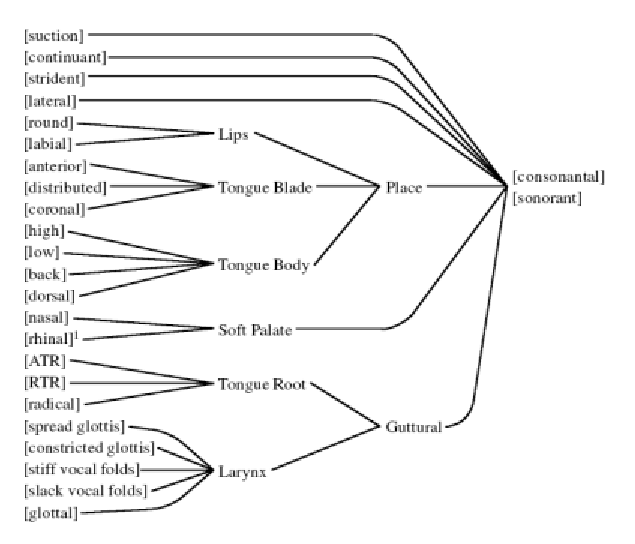
\includegraphics{halle2000feature.geo.v3.eps}
\end{example}

uses xyling\index{xyling} package

\begin{example}\label{singularmorpheme}
Halle-Sagey Style Representation of Shared Features of \textit{singular} /u/\\
\Tree{
&&[-cons]\Below{[+son]}\B[-5]{dll}\B[-5]{drr}\B[-5]{d} \\
Laryngeal\B{d} && Place\B{dl}\B{dr} && [+contin]\\
[voiced] & Dorsal\B{dl}\B{dr} && Labial\B{d} \\
[high] && [back] & [round]\\
~ }
\end{example}
	
	
uses no special packages

\begin{example} Obstruent+Stop clusters\\\label{obststop}
$\left[\begin{array}{l} -son \end{array}\right]\left[\begin{array}{l} -son \\ -cont \\\alpha voice \end{array}\right]\rightarrow\left[\begin{array}{l} -son \\ \alpha voice\end{array}\right]\left[\begin{array}{l} -son \\ -cont\\ \alpha voice\end{array}\right]$
\end{example}

uses no special packages

\begin{example} Obstruent+Fricative clusters\\\label{obstfric}
$\left[\begin{array}{l} -son\end{array}\right]\left[\begin{array}{l} -son \\ +cont\end{array}\right]\rightarrow\left[\begin{array}{l} -son \\ -voice\end{array}\right]\left[\begin{array}{l} -son \\ +cont \\ -voice\end{array}\right]$
\end{example}

	
uses mathmode but no special package

\begin{example}What is the relationship between [a] and [\ipa{O}] ?\\
\begin{description}
\item [Full Specification Approach] ~\\
Change : +low $\rightarrow$ -low, -round $\rightarrow$ +round\\
~[a] : $\left[ \begin{array}{l} +syl\\
+voiced\\
-high\\
+back\\
-ATR\\
+low\\
-round\\
\end{array}\right] $
~[\ipa{O}] :  $\left[ \begin{array}{l} +syl\\
+voiced\\
-high\\
+back\\
-ATR\\
-low\\
+round\\
\end{array}\right] $
\item [Contrastive Specification Approach] ~\\
Change : +low $\rightarrow$ -low\\
Fill : \O high $\rightarrow$ -high, \O back $\rightarrow$ +back, \O ATR $\rightarrow$ -ATR, \O round $\rightarrow$ +round\\
~[a] : $\left[ \begin{array}{l} +syl\\
+low\\
\end{array}\right] $
~[\ipa{O}] :  $\left[ \begin{array}{l} +syl\\
-high\\
+back\\
-ATR\\
-low\\
+round\\
\end{array}\right] $
\end{description}
\end{example}

\subsubsection{Assimilation, Spreading and Feature Specification}

uses xyling\index{xyling} package	
	
\begin{example}\label{placeconstraintrules}
Place Agreement\\
Place of articulation spreads from left to right (indicated by (2)).\\
\Tree{ 
 [+cons]\B{d}_1\B{drr}_2 && [+cons]\B{d}_1 \\
place && place\\
}
\end{example}
uses xyling\index{xyling} package

\begin{example}Anterior Assimilation Rule: Velars\\
\Tree{
(k) & (j)\\
X\ar[u] & X\ar[u]\\
Place\ar[u] & Place\ar[u]\\
Body\ar[u] & Blade\ar[u] \\
[dorsal]\ar[u] & [+anterior]\ar[u]\Linkk[-->]{0}{ul}\\
}
\\Dashed -~- : added link\\
\end{example}

uses xyling\index{xyling} package

\begin{example}\textit{\ipa{n\ae k\textsuperscript{w}\ae s\textsuperscript{j}}} floating Labial [round] and final TH [high] associate\\
$\xymatrix@=6pt{
& X\ar[r] &Oral\ar[r] & (n) \cr
 & X \cr
& X\ar[r] & Oral\ar[r]\ar[rrd] & (k)Dorsal\ar[r] & TT\ar[r] & [back] \cr
 &X& & & \fbox{Labial --[round]}\cr
& X\ar[r] & Oral-(s)\ar[r]\ar[ddr]\ar[ddd] & Dorsal\ar[rr]\ar[rd] & & \fbox{TH --[high]} \cr
 && & & TT\ar[r] & [front] \cr
& && Coronal\ar[r] & Tongue Grove\ar[r] & [grooved] \cr
& &[fricative]\cr
}~$\\
\end{example}

uses pst-autoseg package

\begin{example}Derivation, association, cyclic speading inwards

\vspace{.2in} \index{vspace}
\newpsstyle{assoc}{linestyle=solid,linewidth=.4pt}
\rput[B](0,\asegtsB){k}
\rput[B](1,\asegtsB){i}
\rput[B](2,\asegtsB){l}
\rput[B](3,\asegtsB){i}
\rput[B](4,\asegtsB){f}
\rput[B](5,\asegtsB){o}
\rput[B](6,\asegtsB){k}
\rput[B](7,\asegtsB){a}
\rput[B](8,\asegtsB){f}
\rput[B](9,\asegtsB){o}
\rput[B](1,\asegsyB){L}
\rput[B](3,\asegsyB){H}
\rput[B](9,\asegsyB){H}

\vspace{.2in}
\newpsstyle{assoc}{linestyle=solid,linewidth=.4pt}
\rput[B](0,\asegtsB){k}
\rput[B](1,\asegtsB){i}
\rput[B](2,\asegtsB){l}
\rput[B](3,\asegtsB){i}
\rput[B](4,\asegtsB){f}
\rput[B](5,\asegtsB){o}
\rput[B](6,\asegtsB){k}
\rput[B](7,\asegtsB){a}
\rput[B](8,\asegtsB){f}
\rput[B](9,\asegtsB){o}
\rput[B](1,\asegsyB){L}
\rput[B](3,\asegsyB){H}
\rput[B](9,\asegsyB){H}
\psline[style=assoc](1,\asegtst)(1,\asegsyb)
\psline[style=assoc](3,\asegtst)(3,\asegsyb)
\psline[style=assoc](9,\asegtst)(9,\asegsyb)

\vspace{.2in}
\newpsstyle{assoc}{linestyle=solid,linewidth=.4pt}
\rput[B](0,\asegtsB){k}
\rput[B](1,\asegtsB){i}
\rput[B](2,\asegtsB){l}
\rput[B](3,\asegtsB){i}
\rput[B](4,\asegtsB){f}
\rput[B](5,\asegtsB){o}
\rput[B](6,\asegtsB){k}
\rput[B](7,\asegtsB){a}
\rput[B](8,\asegtsB){f}
\rput[B](9,\asegtsB){o}
\rput[B](1,\asegsyB){L}
\rput[B](3,\asegsyB){H}
\rput[B](9,\asegsyB){H}
\psline[style=assoc](1,\asegtst)(1,\asegsyb)
\psline[style=assoc](3,\asegtst)(3,\asegsyb)
\psline[style=assoc](9,\asegtst)(9,\asegsyb)
\psline[style=assoc](5,\asegtst)(3,\asegsyb)
\psline[style=assoc](7,\asegtst)(9,\asegsyb)

\end{example}

\subsubsection{Prosodic Structures}
uses qtreegina package

 \begin{example}\label{rhyme}Hindi Rhyme configurations (Shukla, 2000)\\
\QTree [.rhyme [.{1 mora} V ] [.{2 mora} V: VC ] [.{3 mora} V:C VCC ] [.{4 mora} V:CC ] ]
\end{example}

uses qtreegina package

\begin{example} $\mu.\mu\mu\mu.\mu\mu.\mu\mu$ : ban\textprimstress du:kba:zi: `marksmanship' 
\QTree[.PrWd [.$\sigma$  [.o b ] [.r  [.$\mu$ a ] [.$\mu$ n ]  ] ] [.$\sigma$ [.o d ] [.r [.$\mu$ u ] [.$\mu$ u ] [.$\mu$ k ] ] ] [.$\sigma$ [.o b ] [.r [.$\mu$ a ] [.$\mu$ a ] ] ] [.$\sigma$ [.o z ] [.r [.$\mu$ i ] [.$\mu$ i ] ] ] ] 
\end{example}



\subsubsection{Stress projection and Tone association}

uses xyling\index{xyling}

\begin{example}\label{manamderivation}
\begin{enumerate}
\item Project vowels
\Treek[0]{0}{
 ~   & L &   & H &   &   & L&   & L &   & L  \cr
 ~ t & a & n & e & p & w & a & t & i & n & a  \cr
}~\\
\item Insert L bracket to the L of H \\
\Treek[0]{0}{
 ~   & L &   & (H &   &   & L&   & L &   & L  \cr
 ~ t & a & n & e & p & w & a & t & i & n & a  \cr
}~\\
\item Iterate: Insert L bracket to the L of pairs \\
\Treek[0]{0}{
 ~   & L &   & (H &   &   & L&   & (L &   & L  \cr
 ~ t & a & n & e & p & w & a & t & i & n & a  \cr
}~\\
\item Head: Left, project head\\
\Treek[0]{0}{
 ~   &  &   & X &   &   & &   & X &   &   \cr
 ~   & L &   & (H &   &   & L&   & (L &   & L  \cr
 ~ t & a & n & e & p & w & a & t & i & n & a  \cr
}~\\
\item Edge: R bracket to the R of the R most element\\
\Treek[0]{0}{
 ~   &  &   & X &   &   & &   & X) &   &   \cr
 ~   & L &   & (H &   &   & L&   & (L &   & L  \cr
 ~ t & a & n & e & p & w & a & t & i & n & a  \cr
}~\\
\item Head: Right, project head\\
\Treek[0]{0}{
 ~   &  &   &  &   &   & &   & X &   &   \cr
 ~   &  &   & X &   &   & &   & X) &   &   \cr
 ~   & L &   & (H &   &   & L&   & (L &   & L  \cr
 ~ t & a & n & e & p & w & a & t & i & n & a  \cr
}~\\
\end{enumerate}
\end{example}



\subsubsection{Optimality Theory}

uses pifont package the hand defined in preamble

as well as color and colortab packages, and the lightgrey  defined in the preamble

as well as the ranking comands fg and og defined in the preamble

\begin{example}
\begin{tabular}{|ll||l|l|l|}\hline
Input: &/kat+z/ & $*\left[\begin{array}{l} -son\\ \alpha voice\end{array}\right]\left[\begin{array}{l} -son\\ -\alpha voice\end{array}\right]$ & IDENT-IO(voice)  & $*\left[\begin{array}{l} -son\\ +voice\end{array}\right]$ \\\hline\hline
\hand & [kats] &  &  * & \\\hline
& [kadz] &  & * & *! *\\
\LCC 
& & & & \color{lightgray} \\\hline
& [gats] & &  * *! & * \\
\ECC
\LCC 
& & & \color{lightgray}& \color{lightgray} \\\hline
& [katz] & *! &  & *\\
\ECC
\LCC 
& & & \color{lightgray}& \color{lightgray} \\\hline
& [kads] & *! &  * * &  * \\\hline
\ECC
\end{tabular}
\end{example}

uses pifont package the hand defined in preamble

as well as the ranking comands fg and og defined in the preamble

\begin{example}
\begin{tabular}{|ll|ccc|ccc|cc|}\hline
 & tanepwtina & *Clash & WSP & Ft & Right & NonFin & Parse & All & Non\\
 & & &  & Bin & most & Stress & Syl& FtR & Fin\\\hline\hline
\hand & ta(n\`{e}pwa)(t\'{i}na) &  &  &  &  &  & * & ** & *\\\hline
 &  (tan\`{e}p)wa(t\'{i}na) &  &  &  &  &  & * & ***! & *\\\hline
 &  ta(n\`{e}pwa)(tin\'{a}) &  &  &  &  & *! & * & ** & *\\\hline
 & ta(n\'{e}pwa)(t\`{i}na) &  &  &  & *! &  & * & ** & *\\\hline
 & (tan\`{e}p)(wat\'{i})na &  &  &  & *! &  & * & **** & \\\hline
 & (ta)(n\`{e}pwa)(t\'{i}na) &  &  & *! &  &  &  & ****** & *\\\hline
 & (t\`{a}nep)wa(t\'{i}na) &  & *! &  &  &  & * & ** & *\\\hline
\end{tabular}
\end{example}

uses pifont package the hand defined in preamble


as well as the ranking comands fg and og defined in the preamble

\begin{example}H Deletion\\ \label{hdeletiontableau}
\begin{tabular}{|lll|l|ccc|l|}\hline
 &  &  &    & *[$_\sigma$h & Max & Onset & No\\
 &  &  &   &  & IO &  & Coda\\\hline\hline
 &  &  & \ipa{/butuh/} &  &  & &\\\hline
MostFaith &  & \hand & \ipa{bu.tUh} &  & & & *\\\hline
LeastMark & MaxIO \fg NoCoda &  & \ipa{bu.tu} & & * &  & \\\hline\hline
 &  &  & \ipa{/butuh/+/e/} & &  &  & \\\hline
 &  & \hand & \ipa{bu.tu.e} & & * & * & \\\hline
MostFaith,LeastMark & *[$_\sigma$h \fg MaxIO,Onset &  & \ipa{bu.tu.he}& * &  &  & \\\hline
\end{tabular}
\end{example}


uses supertabular\index{supertabular} package

as well as the ranking comands fg and og defined in the preamble

\begin{example} A factorial typology of reduplication systems - Kager Ch5,Ex5\\
Five factorial (!5) is 5*4*3*2*1 = 120 different rankings\\
\begin{supertabular}{llllll}
1 & {\sc Align-Red-L} & \fg {\sc Max-BR} & \fg {\sc No-Coda} & \fg {\sc Onset} & \fg {\sc Red}-$\sigma$\\
2 & {\sc Align-Red-L} & \fg {\sc Max-BR} & \fg {\sc No-Coda} & \fg {\sc Red}-$\sigma$ & \fg {\sc Onset}\\
3 & {\sc Align-Red-L} & \fg {\sc Max-BR} & \fg {\sc Onset} & \fg {\sc No-Coda} & \fg {\sc Red}-$\sigma$\\
4 & {\sc Align-Red-L} & \fg {\sc Max-BR} & \fg {\sc Onset} & \fg {\sc Red}-$\sigma$ & \fg {\sc No-Coda}\\
5 & {\sc Align-Red-L} & \fg {\sc Max-BR} & \fg {\sc Red}-$\sigma$ & \fg {\sc Onset} & \fg {\sc No-Coda}\\
6 & {\sc Align-Red-L} & \fg {\sc Max-BR} & \fg {\sc Red}-$\sigma$ & \fg {\sc No-Coda} & \fg {\sc Onset}\\
7 & {\sc Align-Red-L} & \fg {\sc No-Coda} & \fg {\sc Max-BR} & \fg {\sc Onset} & \fg {\sc Red}-$\sigma$\\
8 & {\sc Align-Red-L} & \fg {\sc No-Coda} & \fg {\sc Max-BR} & \fg {\sc Red}-$\sigma$ & \fg {\sc Onset}\\
9 & {\sc Align-Red-L} & \fg {\sc No-Coda} & \fg {\sc Onset} & \fg {\sc Max-BR} & \fg {\sc Red}-$\sigma$\\
10 & {\sc Align-Red-L} & \fg {\sc No-Coda} & \fg {\sc Onset} & \fg {\sc Red}-$\sigma$ & \fg {\sc Max-BR}\\
11 & {\sc Align-Red-L} & \fg {\sc No-Coda} & \fg {\sc Red}-$\sigma$ & \fg {\sc Onset} & \fg {\sc Max-BR}\\
12 & {\sc Align-Red-L} & \fg {\sc No-Coda} & \fg {\sc Red}-$\sigma$ & \fg {\sc Max-BR} & \fg {\sc Onset}\\
13 & {\sc Align-Red-L} & \fg {\sc Onset} & \fg {\sc No-Coda} & \fg {\sc Max-BR} & \fg {\sc Red}-$\sigma$\\
14 & {\sc Align-Red-L} & \fg {\sc Onset} & \fg {\sc No-Coda} & \fg {\sc Red}-$\sigma$ & \fg {\sc Max-BR}\\
15 & {\sc Align-Red-L} & \fg {\sc Onset} & \fg {\sc Max-BR} & \fg {\sc No-Coda} & \fg {\sc Red}-$\sigma$\\
16 & {\sc Align-Red-L} & \fg {\sc Onset} & \fg {\sc Max-BR} & \fg {\sc Red}-$\sigma$ & \fg {\sc No-Coda}\\
17 & {\sc Align-Red-L} & \fg {\sc Onset} & \fg {\sc Red}-$\sigma$ & \fg {\sc Max-BR} & \fg {\sc No-Coda}\\
18 & {\sc Align-Red-L} & \fg {\sc Onset} & \fg {\sc Red}-$\sigma$ & \fg {\sc No-Coda} & \fg {\sc Max-BR}\\
19 & {\sc Align-Red-L} & \fg {\sc Red}-$\sigma$ & \fg {\sc No-Coda} & \fg {\sc Onset} & \fg {\sc Max-BR}\\
20 & {\sc Align-Red-L} & \fg {\sc Red}-$\sigma$ & \fg {\sc No-Coda} & \fg {\sc Max-BR} & \fg {\sc Onset}\\
21 & {\sc Align-Red-L} & \fg {\sc Red}-$\sigma$ & \fg {\sc Onset} & \fg {\sc No-Coda} & \fg {\sc Max-BR}\\
22 & {\sc Align-Red-L} & \fg {\sc Red}-$\sigma$ & \fg {\sc Onset} & \fg {\sc Max-BR} & \fg {\sc No-Coda}\\
23 & {\sc Align-Red-L} & \fg {\sc Red}-$\sigma$ & \fg {\sc Max-BR} & \fg {\sc Onset} & \fg {\sc No-Coda}\\
24 & {\sc Align-Red-L} & \fg {\sc Red}-$\sigma$ & \fg {\sc Max-BR} & \fg {\sc No-Coda} & \fg {\sc Onset}\\
25 & {\sc Max-BR} & \fg {\sc Align-Red-L} & \fg {\sc No-Coda} & \fg {\sc Onset} & \fg {\sc Red}-$\sigma$\\
26 & {\sc Max-BR} & \fg {\sc Align-Red-L} & \fg {\sc No-Coda} & \fg {\sc Red}-$\sigma$ & \fg {\sc Onset}\\
27 & {\sc Max-BR} & \fg {\sc Align-Red-L} & \fg {\sc Onset} & \fg {\sc No-Coda} & \fg {\sc Red}-$\sigma$\\
28 & {\sc Max-BR} & \fg {\sc Align-Red-L} & \fg {\sc Onset} & \fg {\sc Red}-$\sigma$ & \fg {\sc No-Coda}\\
29 & {\sc Max-BR} & \fg {\sc Align-Red-L} & \fg {\sc Red}-$\sigma$ & \fg {\sc Onset} & \fg {\sc No-Coda}\\
30 & {\sc Max-BR} & \fg {\sc Align-Red-L} & \fg {\sc Red}-$\sigma$ & \fg {\sc No-Coda} & \fg {\sc Onset}\\
31 & {\sc Max-BR} & \fg {\sc No-Coda} & \fg {\sc Align-Red-L} & \fg {\sc Onset} & \fg {\sc Red}-$\sigma$\\
32 & {\sc Max-BR} & \fg {\sc No-Coda} & \fg {\sc Align-Red-L} & \fg {\sc Red}-$\sigma$ & \fg {\sc Onset}\\
33 & {\sc Max-BR} & \fg {\sc No-Coda} & \fg {\sc Onset} & \fg {\sc Align-Red-L} & \fg {\sc Red}-$\sigma$\\
34 & {\sc Max-BR} & \fg {\sc No-Coda} & \fg {\sc Onset} & \fg {\sc Red}-$\sigma$ & \fg {\sc Align-Red-L} \\
35 & {\sc Max-BR} & \fg {\sc No-Coda} & \fg {\sc Red}-$\sigma$ & \fg {\sc Onset} & \fg {\sc Align-Red-L} \\
36 & {\sc Max-BR} & \fg {\sc No-Coda} & \fg {\sc Red}-$\sigma$ & \fg {\sc Align-Red-L} & \fg {\sc Onset}\\
37 & {\sc Max-BR} & \fg {\sc Onset} & \fg {\sc No-Coda} & \fg {\sc Align-Red-L} & \fg {\sc Red}-$\sigma$\\
38 & {\sc Max-BR} & \fg {\sc Onset} & \fg {\sc No-Coda} & \fg {\sc Red}-$\sigma$ & \fg {\sc Align-Red-L} \\
39 & {\sc Max-BR} & \fg {\sc Onset} & \fg {\sc Align-Red-L} & \fg {\sc No-Coda} & \fg {\sc Red}-$\sigma$\\
40 & {\sc Max-BR} & \fg {\sc Onset} & \fg {\sc Align-Red-L} & \fg {\sc Red}-$\sigma$ & \fg {\sc No-Coda}\\
41 & {\sc Max-BR} & \fg {\sc Onset} & \fg {\sc Red}-$\sigma$ & \fg {\sc Align-Red-L} & \fg {\sc No-Coda}\\
42 & {\sc Max-BR} & \fg {\sc Onset} & \fg {\sc Red}-$\sigma$ & \fg {\sc No-Coda} & \fg {\sc Align-Red-L} \\
43 & {\sc Max-BR} & \fg {\sc Red}-$\sigma$ & \fg {\sc No-Coda} & \fg {\sc Onset} & \fg {\sc Align-Red-L} \\
44 & {\sc Max-BR} & \fg {\sc Red}-$\sigma$ & \fg {\sc No-Coda} & \fg {\sc Align-Red-L} & \fg {\sc Onset}\\
45 & {\sc Max-BR} & \fg {\sc Red}-$\sigma$ & \fg {\sc Onset} & \fg {\sc No-Coda} & \fg {\sc Align-Red-L} \\
46 & {\sc Max-BR} & \fg {\sc Red}-$\sigma$ & \fg {\sc Onset} & \fg {\sc Align-Red-L} & \fg {\sc No-Coda}\\
47 & {\sc Max-BR} & \fg {\sc Red}-$\sigma$ & \fg {\sc Align-Red-L} & \fg {\sc Onset} & \fg {\sc No-Coda}\\
48 & {\sc Max-BR} & \fg {\sc Red}-$\sigma$ & \fg {\sc Align-Red-L} & \fg {\sc No-Coda} & \fg {\sc Onset}\\
49 & {\sc No-Coda} & \fg {\sc Max-BR} & \fg {\sc Align-Red-L} & \fg {\sc Onset} & \fg {\sc Red}-$\sigma$\\
50 & {\sc No-Coda} & \fg {\sc Max-BR} & \fg {\sc Align-Red-L} & \fg {\sc Red}-$\sigma$ & \fg {\sc Onset}\\
51 & {\sc No-Coda} & \fg {\sc Max-BR} & \fg {\sc Onset} & \fg {\sc Align-Red-L} & \fg {\sc Red}-$\sigma$\\
52 & {\sc No-Coda} & \fg {\sc Max-BR} & \fg {\sc Onset} & \fg {\sc Red}-$\sigma$ & \fg {\sc Align-Red-L} \\
53 & {\sc No-Coda} & \fg {\sc Max-BR} & \fg {\sc Red}-$\sigma$ & \fg {\sc Onset} & \fg {\sc Align-Red-L} \\
54 & {\sc No-Coda} & \fg {\sc Max-BR} & \fg {\sc Red}-$\sigma$ & \fg {\sc Align-Red-L} & \fg {\sc Onset}\\
55 & {\sc No-Coda} & \fg {\sc Align-Red-L} & \fg {\sc Max-BR} & \fg {\sc Onset} & \fg {\sc Red}-$\sigma$\\
56 & {\sc No-Coda} & \fg {\sc Align-Red-L} & \fg {\sc Max-BR} & \fg {\sc Red}-$\sigma$ & \fg {\sc Onset}\\
57 & {\sc No-Coda} & \fg {\sc Align-Red-L} & \fg {\sc Onset} & \fg {\sc Max-BR} & \fg {\sc Red}-$\sigma$\\
58 & {\sc No-Coda} & \fg {\sc Align-Red-L} & \fg {\sc Onset} & \fg {\sc Red}-$\sigma$ & \fg {\sc Max-BR}\\
59 & {\sc No-Coda} & \fg {\sc Align-Red-L} & \fg {\sc Red}-$\sigma$ & \fg {\sc Onset} & \fg {\sc Max-BR}\\
60 & {\sc No-Coda} & \fg {\sc Align-Red-L} & \fg {\sc Red}-$\sigma$ & \fg {\sc Max-BR} & \fg {\sc Onset}\\
61 & {\sc No-Coda} & \fg {\sc Onset} & \fg {\sc Align-Red-L} & \fg {\sc Max-BR} & \fg {\sc Red}-$\sigma$\\
62 & {\sc No-Coda} & \fg {\sc Onset} & \fg {\sc Align-Red-L} & \fg {\sc Red}-$\sigma$ & \fg {\sc Max-BR}\\
63 & {\sc No-Coda} & \fg {\sc Onset} & \fg {\sc Max-BR} & \fg {\sc Align-Red-L} & \fg {\sc Red}-$\sigma$\\
64 & {\sc No-Coda} & \fg {\sc Onset} & \fg {\sc Max-BR} & \fg {\sc Red}-$\sigma$ & \fg {\sc Align-Red-L} \\
65 & {\sc No-Coda} & \fg {\sc Onset} & \fg {\sc Red}-$\sigma$ & \fg {\sc Max-BR} & \fg {\sc Align-Red-L} \\
66 & {\sc No-Coda} & \fg {\sc Onset} & \fg {\sc Red}-$\sigma$ & \fg {\sc Align-Red-L} & \fg {\sc Max-BR}\\
67 & {\sc No-Coda} & \fg {\sc Red}-$\sigma$ & \fg {\sc Align-Red-L} & \fg {\sc Onset} & \fg {\sc Max-BR}\\
68 & {\sc No-Coda} & \fg {\sc Red}-$\sigma$ & \fg {\sc Align-Red-L} & \fg {\sc Max-BR} & \fg {\sc Onset}\\
69 & {\sc No-Coda} & \fg {\sc Red}-$\sigma$ & \fg {\sc Onset} & \fg {\sc Align-Red-L} & \fg {\sc Max-BR}\\
70 & {\sc No-Coda} & \fg {\sc Red}-$\sigma$ & \fg {\sc Onset} & \fg {\sc Max-BR} & \fg {\sc Align-Red-L} \\
71 & {\sc No-Coda} & \fg {\sc Red}-$\sigma$ & \fg {\sc Max-BR} & \fg {\sc Onset} & \fg {\sc Align-Red-L} \\
72 & {\sc No-Coda} & \fg {\sc Red}-$\sigma$ & \fg {\sc Max-BR} & \fg {\sc Align-Red-L} & \fg {\sc Onset}\\
73 & {\sc Onset} & \fg {\sc Max-BR} & \fg {\sc No-Coda} & \fg {\sc Align-Red-L} & \fg {\sc Red}-$\sigma$\\
74 & {\sc Onset} & \fg {\sc Max-BR} & \fg {\sc No-Coda} & \fg {\sc Red}-$\sigma$ & \fg {\sc Align-Red-L} \\
75 & {\sc Onset} & \fg {\sc Max-BR} & \fg {\sc Align-Red-L} & \fg {\sc No-Coda} & \fg {\sc Red}-$\sigma$\\
76 & {\sc Onset} & \fg {\sc Max-BR} & \fg {\sc Align-Red-L} & \fg {\sc Red}-$\sigma$ & \fg {\sc No-Coda}\\
77 & {\sc Onset} & \fg {\sc Max-BR} & \fg {\sc Red}-$\sigma$ & \fg {\sc Align-Red-L} & \fg {\sc No-Coda}\\
78 & {\sc Onset} & \fg {\sc Max-BR} & \fg {\sc Red}-$\sigma$ & \fg {\sc No-Coda} & \fg {\sc Align-Red-L} \\
79 & {\sc Onset} & \fg {\sc No-Coda} & \fg {\sc Max-BR} & \fg {\sc Align-Red-L} & \fg {\sc Red}-$\sigma$\\
80 & {\sc Onset} & \fg {\sc No-Coda} & \fg {\sc Max-BR} & \fg {\sc Red}-$\sigma$ & \fg {\sc Align-Red-L} \\
81 & {\sc Onset} & \fg {\sc No-Coda} & \fg {\sc Align-Red-L} & \fg {\sc Max-BR} & \fg {\sc Red}-$\sigma$\\
82 & {\sc Onset} & \fg {\sc No-Coda} & \fg {\sc Align-Red-L} & \fg {\sc Red}-$\sigma$ & \fg {\sc Max-BR}\\
83 & {\sc Onset} & \fg {\sc No-Coda} & \fg {\sc Red}-$\sigma$ & \fg {\sc Align-Red-L} & \fg {\sc Max-BR}\\
84 & {\sc Onset} & \fg {\sc No-Coda} & \fg {\sc Red}-$\sigma$ & \fg {\sc Max-BR} & \fg {\sc Align-Red-L} \\
85 & {\sc Onset} & \fg {\sc Align-Red-L} & \fg {\sc No-Coda} & \fg {\sc Max-BR} & \fg {\sc Red}-$\sigma$\\
86 & {\sc Onset} & \fg {\sc Align-Red-L} & \fg {\sc No-Coda} & \fg {\sc Red}-$\sigma$ & \fg {\sc Max-BR}\\
87 & {\sc Onset} & \fg {\sc Align-Red-L} & \fg {\sc Max-BR} & \fg {\sc No-Coda} & \fg {\sc Red}-$\sigma$\\
88 & {\sc Onset} & \fg {\sc Align-Red-L} & \fg {\sc Max-BR} & \fg {\sc Red}-$\sigma$ & \fg {\sc No-Coda}\\
89 & {\sc Onset} & \fg {\sc Align-Red-L} & \fg {\sc Red}-$\sigma$ & \fg {\sc Max-BR} & \fg {\sc No-Coda}\\
90 & {\sc Onset} & \fg {\sc Align-Red-L} & \fg {\sc Red}-$\sigma$ & \fg {\sc No-Coda} & \fg {\sc Max-BR}\\
91 & {\sc Onset} & \fg {\sc Red}-$\sigma$ & \fg {\sc No-Coda} & \fg {\sc Align-Red-L} & \fg {\sc Max-BR}\\
92 & {\sc Onset} & \fg {\sc Red}-$\sigma$ & \fg {\sc No-Coda} & \fg {\sc Max-BR} & \fg {\sc Align-Red-L} \\
93 & {\sc Onset} & \fg {\sc Red}-$\sigma$ & \fg {\sc Align-Red-L} & \fg {\sc No-Coda} & \fg {\sc Max-BR}\\
94 & {\sc Onset} & \fg {\sc Red}-$\sigma$ & \fg {\sc Align-Red-L} & \fg {\sc Max-BR} & \fg {\sc No-Coda}\\
95 & {\sc Onset} & \fg {\sc Red}-$\sigma$ & \fg {\sc Max-BR} & \fg {\sc Align-Red-L} & \fg {\sc No-Coda}\\
96 & {\sc Onset} & \fg {\sc Red}-$\sigma$ & \fg {\sc Max-BR} & \fg {\sc No-Coda} & \fg {\sc Align-Red-L} \\
97 & {\sc Red}-$\sigma$ & \fg {\sc Max-BR} & \fg {\sc No-Coda} & \fg {\sc Onset} & \fg {\sc Align-Red-L} \\
98 & {\sc Red}-$\sigma$ & \fg {\sc Max-BR} & \fg {\sc No-Coda} & \fg {\sc Align-Red-L} & \fg {\sc Onset}\\
99 & {\sc Red}-$\sigma$ & \fg {\sc Max-BR} & \fg {\sc Onset} & \fg {\sc No-Coda} & \fg {\sc Align-Red-L} \\
100 & {\sc Red}-$\sigma$ & \fg {\sc Max-BR} & \fg {\sc Onset} & \fg {\sc Align-Red-L} & \fg {\sc No-Coda}\\
101 & {\sc Red}-$\sigma$ & \fg {\sc Max-BR} & \fg {\sc Align-Red-L} & \fg {\sc Onset} & \fg {\sc No-Coda}\\
102 & {\sc Red}-$\sigma$ & \fg {\sc Max-BR} & \fg {\sc Align-Red-L} & \fg {\sc No-Coda} & \fg {\sc Onset}\\
103 & {\sc Red}-$\sigma$ & \fg {\sc No-Coda} & \fg {\sc Max-BR} & \fg {\sc Onset} & \fg {\sc Align-Red-L} \\
104 & {\sc Red}-$\sigma$ & \fg {\sc No-Coda} & \fg {\sc Max-BR} & \fg {\sc Align-Red-L} & \fg {\sc Onset}\\
105 & {\sc Red}-$\sigma$ & \fg {\sc No-Coda} & \fg {\sc Onset} & \fg {\sc Max-BR} & \fg {\sc Align-Red-L} \\
106 & {\sc Red}-$\sigma$ & \fg {\sc No-Coda} & \fg {\sc Onset} & \fg {\sc Align-Red-L} & \fg {\sc Max-BR}\\
107 & {\sc Red}-$\sigma$ & \fg {\sc No-Coda} & \fg {\sc Align-Red-L} & \fg {\sc Onset} & \fg {\sc Max-BR}\\
108 & {\sc Red}-$\sigma$ & \fg {\sc No-Coda} & \fg {\sc Align-Red-L} & \fg {\sc Max-BR} & \fg {\sc Onset}\\
109 & {\sc Red}-$\sigma$ & \fg {\sc Onset} & \fg {\sc No-Coda} & \fg {\sc Max-BR} & \fg {\sc Align-Red-L} \\
110 & {\sc Red}-$\sigma$ & \fg {\sc Onset} & \fg {\sc No-Coda} & \fg {\sc Align-Red-L} & \fg {\sc Max-BR}\\
111 & {\sc Red}-$\sigma$ & \fg {\sc Onset} & \fg {\sc Max-BR} & \fg {\sc No-Coda} & \fg {\sc Align-Red-L} \\
112 & {\sc Red}-$\sigma$ & \fg {\sc Onset} & \fg {\sc Max-BR} & \fg {\sc Align-Red-L} & \fg {\sc No-Coda}\\
113 & {\sc Red}-$\sigma$ & \fg {\sc Onset} & \fg {\sc Align-Red-L} & \fg {\sc Max-BR} & \fg {\sc No-Coda}\\
114 & {\sc Red}-$\sigma$ & \fg {\sc Onset} & \fg {\sc Align-Red-L} & \fg {\sc No-Coda} & \fg {\sc Max-BR}\\
115 & {\sc Red}-$\sigma$ & \fg {\sc Align-Red-L} & \fg {\sc No-Coda} & \fg {\sc Onset} & \fg {\sc Max-BR}\\
116 & {\sc Red}-$\sigma$ & \fg {\sc Align-Red-L} & \fg {\sc No-Coda} & \fg {\sc Max-BR} & \fg {\sc Onset}\\
117 & {\sc Red}-$\sigma$ & \fg {\sc Align-Red-L} & \fg {\sc Onset} & \fg {\sc No-Coda} & \fg {\sc Max-BR}\\
118 & {\sc Red}-$\sigma$ & \fg {\sc Align-Red-L} & \fg {\sc Onset} & \fg {\sc Max-BR} & \fg {\sc No-Coda}\\
119 & {\sc Red}-$\sigma$ & \fg {\sc Align-Red-L} & \fg {\sc Max-BR} & \fg {\sc Onset} & \fg {\sc No-Coda}\\
120 & {\sc Red}-$\sigma$ & \fg {\sc Align-Red-L} & \fg {\sc Max-BR} & \fg {\sc No-Coda} & \fg {\sc Onset}\\
\end{supertabular}
\end{example}


\subsection{Morphology}

\subsubsection{Architecture of the grammar}

uses xyling\index{xyling} package

\begin{example}
\fbox{
\xymatrix{
Lexicon\ar[dd] &  \cr
\ar@/^1pc/[dr] &  {\textit{Spell-out}}\cr
LF & PF \cr
}}
\end{example}

uses qtreegina  package

\begin{example}\label{discripfreqschemata}
Arrernte Frequentive Forms\\
$verb + ep + final syllable + em$\\
\QTree[ [ [ [.verb root\\unt v\textsuperscript{o}\\\ipa{\o} ] atelic\\ep ] freq\\unt ] prog\\em ]
\end{example}


\subsubsection{Precedence Theory Phonology-Morphology Interface}

uses xyling\index{xyling} package

\begin{example}Final syllable precedes stressed syllable\\\label{manamprecedence}
\hspace{1in} \xymatrix{
~\#\ar[r] & X\ar[r] & \sigma_{A+stress}\ar[r]  & Y\ar[r] & \sigma_{Bn}\ar@/^1.5pc/[ll]\ar[r] & ~\% \cr
}
~\\~\\
(Where $X$ and $Y$ represent a sequence of $0+$ atoms.)
\end{example} 

uses xyling\index{xyling} package

\begin{example} \textit{\ipa{g\textsuperscript{w}@z\textsuperscript{j}}} /gz/ `cut \dots', Labial [round] \& TH [high] `feminine', reduplicated  \\
$\xymatrix@=6pt{	
& ~\#\ar[d] \cr
& X\ar[r]\ar[d] & Oral\ar[r] & (g)Dorsal\ar[r]\ar[rd] & TT\ar[r] & [back]\\
 & X\ar[d] &&& \fbox{Labial --[round]}\cr
& X\ar[r]\ar[d]\ar@/^2.5pc/[uu] & Oral\ar[r] & (z)Dorsal\ar[r]\ar[dr] & TT\ar[r] & [front] \\
& ~\%&&& \fbox{TH --[high]}\cr 	
}~$\\
\end{example}

uses xyling\index{xyling}

\begin{example}Derivation of Frequentive Forms\\\label{freqderivation}
\begin{enumerate}
\item Verb
\xymatrix{
 ~\#\ar[r] & e\ar[r] & m\ar[r] & p\textsuperscript{w}\ar[r] & a\ar[r] & r\ar[r]   & ~\% \cr
}~\\
\item Suffix ep
\xymatrix{
 ~\#\ar[r] & e\ar[r] & m\ar[r] & p\textsuperscript{w}\ar[r] & a\ar[r] & r\ar[r]\ar[d]   & ~\% \cr
 &  & & &  & e\ar[d] & \cr
 &  & & &  & p &
}~\\
\item Final segment precedes Final syllable
\xymatrix{
 ~\#\ar[r] & e\ar[r] & m\ar[r] & p\textsuperscript{w}\ar[r] & a\ar[r] & r\ar[r]\ar[d]   & ~\% \cr
 &  & & & p\ar@/^1.5pc/[u] & e\ar[l] &
}~\\
\item Suffix em
\xymatrix{
 & & & & & e\ar[r] & m\ar[d]\cr
 ~\#\ar[r] & e\ar[r] & m\ar[r] & p\textsuperscript{w}\ar[r] & a\ar[r] & r\ar[r]\ar[d]\ar[u]   & ~\% \cr
 &  & & & p\ar@/^1.5pc/[u] & e\ar[l] &
}~\\
\end{enumerate}
\end{example} 


\subsection{Syntax}
	
\subsubsection{John Frampton's trees}

uses pst-jtree, pst-xkey and pstricks packages

see jtree documentation

\jtree
\! = :{a} :{b} :{c} :{d} {e}.
\endjtree


\jtree[xunit=2.8em,yunit=1em]
\! = {S}
:{NP}!a {VP}
:{V}!b {NP}
<vert>{Tom}.
\!a = <vert>{Mary}.
\!b = <vert>{saw}.
\endjtree


\jtree
\! = :{\rnode{A1}{who}}
:{\rnode{B1}{did}} :{Jack}
:{\rnode{B2}{\sl t}} :{see}
{\rnode{A2}{\sl t}}.
\psset{arrows=->,angleA=-150,
angleB=-90}
\nccurve{A2}{A1}
\nccurve{B2}{B1}
\endjtree


\jtree
\! = :{a}!a (:{b}{c}){d}.
\endjtree


\jtree
\def\fracture{\psframebox{Fracture}}
\! = {\stuff[a]}
<vert>{\fracture}
:\jtbig{\stuff[b]}!a
\jtbig{\stuff[c]}
<vert>{\fracture}
:{$\vdots$} {$\vdots$}.
\endjtree

\jtree[xunit=2.6em,yunit=1em]
\def\\{[labelgapb=-1.2ex]}% 1
\everymath={\rm}%
\! = {CP}
:({XP}\\{$\scriptstyle [wh]$}@A1 ) {$C�$}
:({$C�0$}\\{$\scriptstyle [wh,Q]$})
{$\langle\, TP\,\rangle$}
<tri>{\dots\quad\rnode[b]{A2}{\it t}\quad\dots}. 2
\nccurve[angleA=-150,angleB=-90,ncurv=1]{->}{A2}{A1}
\endjtree


\subsubsection{xyling\index{xyling} tree templates for copying}

uses xyling\index{xyling} package

\begin{example}Head Final Structure for copying \\
\Treek{1}{ 
& TP\B{dl}\B{dr}\\
DP && '\B{dl}\B{dr} \\
& P\B{dl}\B{dr}&&^o\\
DP && '\B{dl}\B{dr} \\
& P&&^o\\
}

\end{example}

uses xyling\index{xyling} package

\begin{example}Head Initial Structure for copying\\
\Treek{1}{ 
& TP\B{dl}\B{dr}\\
DP  && '\B{dl}\B{dr} \\
& ^o&&P\B{dl}\B{dr}\\
&&DP && '\B{dl}\B{dr} \\
&& & ^o&&P\B{dl}\B{dr}\\
&& &&DP && '\B{dl}\B{dr} \\
&& && & ^o&&P\B{dl}\B{dr}\\
&& && &&DP && '\B{dl}\B{dr} \\
&& && &&  & ^o&&P\B{dl}\B{dr}\\
&& && && &&  DP && '\B{dl}\B{dr} \\
&& && && &&  & ^o&&P\\
}

\end{example}
\subsubsection{Changing spacing in the tree}

uses xyling\index{xyling} package

\begin{example}Default space\\
\Tree{ 
& TP\B{dl}\B{dr}\\
DP && '\B{dl}\B{dr} \\
& P\B{dl}\B{dr}&&^o\\
DP && '\B{dl}\B{dr} \\
& P&&^o\\
}
\end{example} 


You can use Treek to change the vertical spacing, put its argument in curly braces \begin{verbatim} \Treek{3} \end{verbatim}

uses xyling\index{xyling} package

\begin{example} 3 space \\
\Treek{3}{ 
& TP\B{dl}\B{dr}\\
DP && '\B{dl}\B{dr} \\
& P\B{dl}\B{dr}&&^o\\
DP && '\B{dl}\B{dr} \\
& P&&^o\\
}
\end{example}

You can also change the horizontal spacing with an optional argument in square brackets in either Tree (the default vertical spacing) or Treek (a specified vertical spacing) \begin{verbatim} \Treek[4]{3} or \Tree[4] \end{verbatim}

uses xyling\index{xyling} package

\begin{example} 3 space, with 4 wide \\
\Treek[4]{3}{ 
& TP\B{dl}\B{dr}\\
DP && '\B{dl}\B{dr} \\
& P\B{dl}\B{dr}&&^o\\
DP && '\B{dl}\B{dr} \\
& P&&^o\\
}
\end{example}

\subsubsection{Complicated tree samples}

These examples were made from looking at the xyling\index{xyling} documentation. 

uses xyling\index{xyling} package

\begin{example} 
Raising for Case\\
\begin{tabular}{ll}
\Treek{1}{ 
\K{a) Turkish }\\
& TP\B{dl}\B{dr}\\
\K{~~~~~~~Subj$_{nom}$} && T'\B{dl}\B{dr} \\
& vP\B{dl}\B{dr}&&\K{$V^o+v^o+T^o$~~~~~~~~~~~~}\Linkk[<--]{1.8}{rddd}\\
\K{~~~~~~~Obj$_{acc}$} && v'\B{dl}\B{dr} \QS{2,1}{5,4} \QS[.]{6,2}{12,5}&\\
&Subj\Below{Ali}\Linkk[>]{1.8}{luuu} && v'\B{dl}\B{dr} \\
&& VP\B{dl}\B{dr}&&\K{$V^o+v^o$~~~~~}\Linkk[<--]{1.8}{dd}\\
& && V'\B{dl}\B{dr} \\
&& VP\B{dl}\B{dr}&&V^o\Below{want}\\
& && V'\B{dl}\B{dr} \\
&&Obj\Below{one piano}\Linkk[>]{2.5}{lluuuuuu}&&V^o\Below{rent}\\
&& && \\
}
&

\Treek[-1]{1}{ 
\K{b) Spanish}\\
& TP\B{dl}\B{dr} &&&& && &&& \hspace{-.8in}Restricted~Clause\\
\K{~~~~~~~Subj$_{nom}$}  && T'\B{dl}\B{dr} \\
& \K{$V^o+v^o+T^o$}&&vP\B{dl}\B{dr}\\
&&\K{Obj$_{acc}$} && v'\B{dl}\B{dr} \QS{2,1}{5,4} \QS[.]{6,4}{12,11} \\
&& & Subj\Below{~~~Griselda}\Linkk[>]{4.5}{llluuu}&&v'\B{dl}\B{dr}  && &&&\hspace{-.8in}Nuclear~Scope\\
&& &&  \K{$V^o+v^o$}\Linkk[-->]{4.5}{llluuu}&&VP\B{dl}\B{dr}\\
&& && & && V'\B{dl}\B{dr} \\
&& && &&   V^o\Below{want}\Linkk[-->]{2.5}{lluu}&&VP\B{dl}\B{dr}\\
&& && && &   && V'\B{dl}\B{dr} \\
&& && && &&   V^o\Below{invite}&& Obj\Below{a doctor~~~~}\Linkk[>]{8.5}{lllllllluuuuuu}\\
&& && && && &&\\
}
\end{tabular}
\end{example}


\begin{example} 
Case Triggers Raising\\
\begin{tabular}{ll}
\Treek{1}{ 
\K{a) Turkish }\\
& TP\B{dl}\B{dr}\\
\K{~~~~~~~Subj$_{nom}$} && T'\B{dl}\B{dr} \\
& vP\B{dl}\B{dr}&&\K{$V^o+v^o+T^o$~~~~~~~~~~~~}\Linkk[<--]{1.8}{rddd}\\
\K{~~~~~~~Obj$_{acc}$} && vPx\B{dl}\B{dr} \QS{2,1}{5,4} \QS[.]{6,2}{12,5}&\\
&Subj\Below{Ali}\Linkk[>]{1.8}{luuu} && v'\B{dl}\B{dr} \\
&& VP\B{dl}\B{dr}&&\K{$V^o+v^o$~~~~~}\Linkk[<--]{1.8}{dd}\\
& && V'\B{dl}\B{dr} \\
&& VP\B{dl}\B{dr}&&V^o\Below{want}\\
& && V'\B{dl}\B{dr} \\
&&\K{Obj$_{acc}$}\Below{one piano}\Linkk[>]{2.5}{lluuuuuu}&&V^o\Below{rent}\\
&& && \\
}

&

\Treek[-1]{1}{ 
\K{b) Spanish}\\
& TP\B{dl}\B{dr} &&&& && &&& \hspace{-.8in}Restricted~Clause\\
\K{~~~~~~~Subj$_{nom}$}  && T'\B{dl}\B{dr}\\
& \K{$V^o+v^o+T^o$}&&vP\B{dl}\B{dr}\\
&&\K{Obj$_{acc}$} && vP\B{dl}\B{dr} \QS{2,1}{5,4} \QS[.]{6,4}{12,11} \\
&& & Subj\Below{~~~Griselda}\Linkk[>]{4.5}{llluuu}&&v'\B{dl}\B{dr}&& &&&\hspace{-.8in}Nuclear~Scope\\
&& &&  \K{$V^o+v^o$}\Linkk[-->]{4.5}{llluuu}&&VP\B{dl}\B{dr}\\
&& && & && V'\B{dl}\B{dr} \\
&& && &&   V^o\Below{want}\Linkk[-->]{2.5}{lluu}&&VP\B{dl}\B{dr}\\
&& && && &   && V'\B{dl}\B{dr} \\
&& && && &&   V^o\Below{invite}&& \K{Obj$_{acc}$~~~~~~~}\Below{a doctor~~~~}\Linkk[>]{8.5}{lllllllluuuuuu}\\
&& && && && &&\\
}
\end{tabular}
\end{example}


\subsubsection{Discourse representation theory}

uses covington package

\drs{X}
{named(X,�Pedro�) \\
\drs{Y}{donkey(Y)\\owns(X,Y)}~~
{\large $\Rightarrow$}~
\drs{~}{feeds(X,Y)}
}



\subsection{Semantics}

uses the denotation brackets that are in the preamble (some people use the stmarysrd package, but this definition makes the denotation bold, and is simpler to declare)

uses the qtreegina package

\begin{example}Sample denotation brackets

\denoteexpand{\QTree [ Ann walks ]} = (\denote{Ann})\denote{walks}
\end{example}

uses the xyling\index{xyling} package

\begin{example}Semantic Combination under Functional Application (FA)\\
\label{FA}
\Tree{
& \denote{\gamma}\Below{$_\textsc{fa}$}\B{dl}\B{dr} &&  =\denote{\alpha}(\denote{\beta})\\
\denote{\alpha} && \denote{\beta}\\
}
\end{example}

uses the xyling\index{xyling} package


\begin{example}Typical example of Functional Appilcation (FA)\\
\label{typicalFA}
\begin{tabular}{ll}
\Tree[-1]{
\K{(a) English}\\
& VP_{<e,t>}\Below{$_\textsc{fa}$}\B{dl}\B{dr} &&  =\denote{hug}(\denote{NP})\\
{V}_{<e,<e,t>>}\Below{\denote{hug}} && NP_e\Below{\denote{Mary}}\\
}&
\Tree[-1]{
\K{(b) Turkish} \\
& VP_{<e,t>}\Below{$_\textsc{fa}$}\B{dl}\B{dr} && \hspace{-.2in} =(\denote{NP-e})\denote{sardil-di}\\
NP_e\Below{\denote{Mary-e}} && {V}_{<e,<e,t>>}\Below{\denote{sarid-di}}\\
}
\end{tabular}
\end{example}

uses the xyling\index{xyling} package

\begin{example}Semantic Combination under Intersection (a.k.a. Predicate Modification)\\
\label{PM}
\Tree{
& \denote{\gamma}\Below{$_\cap$}\B{dl}\B{dr} &&  =\denote{\alpha} \cap \denote{\beta}\\
\denote{\alpha} && \denote{\beta}\\
}
\end{example}


uses the xyling\index{xyling} package

\begin{example}Typical example of Intersection/Predicate Modification($\cap$/PM)\\
\Tree{
& NP_{<e,t>}\Below{$_\cap$}\B{dl}\B{dr} &&  =\denote{Adj} \cap \denote{NP}\\
{AdjP}_{<e,t>}\Below{\denote{blue}} && NP_{<e,t>}\Below{\denote{ball}}\\
}
\end{example}

uses the PSTricks and pst-grad packages

\begin{example}The Intersection Generalization: Adjectives\\
\label{intersectgenadj}
(i) English Example: \\
Assumption: $\gamma$ is an Individual\\
If $\gamma$ is a wuggy ball (where wuggy stands for any adjective), then\\
\hspace{.2in}it is necessarily the case that $\gamma$ is wuggy and,\\
\hspace{.2in}it is necessarily the case that $\gamma$ is a ball.\\
(ii) This can be modelled logically as:\\
Assumption: $\gamma \in D_{individuals}$ \\
$\gamma \in (\denote{Adjective} \cap \denote{Noun})$\\
\hspace{.2in}$\models \gamma \in \denote{Adjective} $\\
\hspace{.2in}$\models \gamma \in \denote{Noun} $\\
(iii) In words: If $\gamma$ is a member of the intersection of sets \denote{Adjective} and \denote{Noun}, then\\
\hspace{.2in}it is necessarily the case that $\gamma$ is a member of \denote{Adjective} and \\
\hspace{.2in}it is necessarily the case that$\gamma$ is a member of \denote{Noun}.
\psset{linestyle=solid}
\psset{unit=3em} % gets the right unit size, pst-autoseg interferes with it
 %\psgrid(0,0)(-1,-1)(9,4.5)
 \pscircle(4.5,3){1}
 \pscircle(6,3){1}
   \uput[0](3.5,3){\psframebox*{$\denote{Adj}$}}
   \uput[0](5.4,3){$\denote{Noun}$}
  \uput[0](5,3){$\gamma$}
\uput[0](3,4){(iv)}

\end{example}

uses xyling\index{xyling} package

\begin{example}Adverbs have two possible places of attachment\\
\label{syntaxforadverbials}
\Treek{1}{
\K{(a) Attached to VP}\\
&& S\B{dl}\B{dr}\\
&Subj && VP\B{dl}\B{dr}\\
&&VP\B{dl}\B{dr}\OO && Adv\\
&V && Obj\\
}
\Treek{1}{
\K{(b) Attached to S}\\
&&& S\B{dl}\B{dr}\\
&& S\B{dl}\B{dr}\OO && Adv\\
&Subj && VP\B{dl}\B{dr}\\
 &&V && Obj\\
}
\end{example}


uses xyling\index{xyling} package

\begin{example}Tense is easy to add via Intersection\\
\Tree{
 & TP_{\{e\}}\Below{$_\cap$}\B{dl}\B{dr}&&&&&&& \K{ = \{e:  John is an agent of e $\cap$ e is a running event $\cap$ e happened in the past\}}  \\
T_{\{e\}}\Below{Past} &&  VP_{\{e\}}\B{dl}\B{dr} &&&&& \K{ = \{e:  John is an agent of e $\cap$ e is a running event\}}  \\
 & {NP}\Below{\denote{John}} && VP\Below{\denote{ran}}\\
}
\end{example}

uses the PSTricks and pst-grad packages \index{set theory}


\begin{example}Extra-Linguistic Solution: A sentence is true if the sets of events is non-empty\\
\label{trueevents}
(i) Situation:\\
\hspace{.2in}D = \{e$_1$,e$_2$,e$_3$,e$_4$,e$_5$,e$_6$\}\\
\hspace{.2in}John is an agent = \{e$_1$,e$_4$,e$_5$\}\\
\hspace{.2in}run = \{e$_1$,e$_3$,e$_5$\}\\
\hspace{.2in}quickly = \{e$_1$,e$_2$,e$_5$\}\\
\hspace{.2in}swim = \{e$_6$\}\\

%\makebox[\textwidth]{\framebox[5cm]{\rule{0pt}{4cm}}}
\vspace{.4in}
\psset{unit=3em} % gets the right unit size, pst-autoseg interferes with it
\psset{linestyle=solid}
 %\psgrid(0,0)(-1,-1)(11,3)
 \pscircle(8,2){1.5}
 \pscircle(7.5,1){1.5}
 \pscircle(9,1){1.5}
   \uput[0](7,3){\psframebox*{John}}
   \uput[0](6,1){\psframebox*{running}}
   \uput[0](8.9,.8){quickly}
 %\psdot*[dotstyle=diamond,fillcolor=blue,dotsize=2pt 8](8,2)
 %\psdot*[dotstyle=square,fillcolor=blue,dotsize=2pt 8](10,2.5)
 \uput[0](8,1){e$_1$}
 \uput[135](10,1.5){e$_2$}
 \uput[135](7,0){e$_3$}
  \uput[0](8,2.5){e$_4$}
  \uput[0](8,1.3){e$_5$}
  \uput[0](10,2.5){e$_6$}
\uput[0](5.5,2.5){(iii)}

\vspace{-.5in}
(ii) Derivation\\
\denote{John ran quickly} \\
\hspace{.2in} = John $\cap$ run $\cap$ quick\\
\hspace{.2in} = \{e$_1$,e$_4$,e$_5$\} $\cap$ \{e$_1$,e$_3$,e$_5$\} $\cap$ \{e$_1$,e$_2$,e$_5$\}\\
\hspace{.2in} = \{e$_1$,e$_5$\}\\
\hspace{.2in} (= True)
\end{example}

uses xyling\index{xyling} package

\begin{example}Again can also attach to a VP\\
\label{transVPagain}
\begin{tabular}{ll}
Normal Example & Context Driven Example\\\hline
John hugged Mary because she looked sad, & John's wife hugged Mary because she looked sad,\\
She still looked sad so & She still looked sad so \\
\\
(a) [John hugged Mary] again. & (b) John [hugged Mary] again.\\
\Tree{
&& S_{\{e\}}\Below{$_\cap$}\B{dl}\B{dr} && \\
&S_{\{e\}}\OO\B{dl}\B{dr} && Adv_{\{e\}}\Below{again}\\
NP_{\{e\}}\Below{John} && VP_{\{e\}}\B{dl}\B{dr}\\
&V\Below{hugged}&& NP\Below{Mary}\\
} &
\Tree{
&S_{\{e\}}\Below{$_\cap$}\B{dl}\B{dr} &&\\
NP_{\{e\}}\Below{John} && VP_{\{e\}}\Below{$_\cap$}\B{dl}\B{dr}\\
&VP_{\{e\}}\OO\B{dl}\B{dr} && Adv_{\{e\}}\Below{again}\\
V\Below{hugged}&& NP\Below{Mary}\\
}\\
\end{tabular}
\end{example}
\section{Some examples of how to site from a bibtex bibliography}

\citet{Ormazabal:2007}



\citet[Chap.~3]{Diesing:1992}

\citet[: 78]{Diesing:1992}

\citet{Epstein:1996}

\citet*{Epstein:1996}

\citep{Lasnik:1977}


% \section{References}

\bibliography{bibliography071218}


%\section{Index}

\printindex
%latex the file once, then run this at the commandline in the same directory: makeindex  latex.examples-gina.v5.ist


\end{document}
